\documentclass{beamer}

% macros file
%% packages

% bibliography
\usepackage{cite}
\usepackage[nottoc]{tocbibind}

% subfiles structure
\usepackage{subfiles}

% fonts
\usepackage[T1]{fontenc}
\usepackage[utf8]{inputenc}

% ams stuff
\usepackage{amsthm, amsmath, amssymb, amsfonts}

% physics
\usepackage{physics}

% bold math
\usepackage{bbold, bm, bbm}

% various letters for enumerate fields
\usepackage{enumitem}

% if statments
\usepackage{xifthen}

% graphics
\usepackage{graphicx, float}

% making figures in tex
\usepackage{tikz, pgfplots}
    \pgfplotsset{compat=1.9}   

%% math commands

% sign of value
\newcommand{\sgn}[1]{\mathrm{sgn}\left( #1 \right)}

% function support
\newcommand{\supp}[1]{\mathrm{supp}\left( #1 \right)}

% vectors and vector spaces
\renewcommand{\vec}[1]{\bm{#1}}
\renewcommand{\norm}[1]{\left|\left| #1 \right|\right|}
\newcommand{\inner}[1]{\left\langle #1 \right\rangle}

% special functions
\renewcommand{\exp}[1]{\text{exp}\left(#1\right)}
\renewcommand{\log}[1]{
		\mathrm{log}\left( #1 \right)
}

% specify path relative to main.tex
%\renewcommand{\sin}[2][1]{
    \mathrm{sin}^{
        \ifthenelse{\equal{#1}{1}}{}{\,#1}
    }
    \left( #2 \right)
}
\renewcommand{\cos}[2][1]{
    \mathrm{cos}^{
        \ifthenelse{\equal{#1}{1}}{}{\,#1}
    }
    \left( #2 \right)
}
\renewcommand{\cot}[1]{\mathrm{cot}\left( #1 \right)}
\renewcommand{\cosh}[2][1]{
    \mathrm{cosh}^{
        \ifthenelse{\equal{#1}{1}}{}{\,#1}
    }
    \left( #2 \right)
}
\renewcommand{\sinh}[2][1]{
    \mathrm{sinh}^{
        \ifthenelse{\equal{#1}{1}}{}{\,#1}
    }
    \left( #2 \right)
}
\renewcommand{\tanh}[1]{
		\mathrm{tanh}\left( #1 \right)
}
\renewcommand{\tan}[1]{
		\mathrm{tan}\left( #1 \right)
}
\newcommand{\sech}[2][1]{
		\mathrm{sech}^{
				\ifthenelse{\equal{#1}{1}}{}{\,#1}
		}
		\left( #2 \right)
}
\newcommand{\asin}[1]{
		\mathrm{arcsin}\left( #1 \right)
}
\newcommand{\acos}[1]{
		\mathrm{arccos}\left( #1 \right)
}
\newcommand{\atan}[1]{
		\mathrm{arctan}\left( #1 \right)
}





% sets
\newcommand{\R}{\mathbb{R}}
\newcommand{\C}{\mathbb{C}}
\newcommand{\N}{\mathbb{N}}
\newcommand{\Z}{\mathbb{Z}}

% derivatives
% specify path relative to main.tex
\usepackage{xifthen}

\renewcommand{\vec}[1]{\mathbf{#1}}

\newcommand{\der}[3][1]{
	\frac{{\text{d}^{
		\ifthenelse{\equal{#1}{1}}{}{\,#1}
	}
	{#2} }}
	{\text{d} {#3}^{
		\ifthenelse{\equal{#1}{1}}{}{#1}
	}
	}
}

\newcommand{\pder}[3][1]{
	\frac{\partial^{
		\ifthenelse{\equal{#1}{1}}{}{\,#1}
	}
	{#2}}
	{\partial {#3}^{
		\ifthenelse{\equal{#1}{1}}{}{#1}
	}
	}
}

% functional stuff
\newcommand{\embeds}{\hookrightarrow}

% probability
\newcommand{\E}[2][1]{
		\mathbb E_{
				\ifthenelse{\equal{#1}{1}}{}{#1}
		} \left[ #2 \right]
}
\renewcommand{\P}{\mathbb P}
%\newcommand{\var}[1]{
%		\mathrm{Var}\left( #1 \right)
%}
\newcommand{\relent}[2]{
		D_\mathrm{KL} \left(
		#1 \mid \mid #2 \right)
}


% page setup
\everymath{\displaystyle}
\usepackage[margin=1in]{geometry}



\title[FEM for Quantum]{
		Finite Element Method for Quantum Mechanics
}

\author[J. Troy]{Jerome Troy}
\date{May 13, 2021}

\begin{document}

\begin{frame}
		\titlepage
\end{frame}

\begin{frame}{An Overview of Quantum Mechanics}
  \begin{itemize}
  	\item \textbf{Heisenberg Uncertainty Principle} : ``
			You cannot simultaneously know the position and 
			momentum of a quantum particle''
	\item Classical rules $\vec F = m \vec a$ are changed to
			quantum rules: \textbf{Sch\"odinger Equation}
			\[
					i \hbar \pder{\Psi}{t} = \hat H\left[\Psi\right]
			\] 
	\item $\hbar$ - Planck's Constant (divided by $2\pi$), 
			$\hat H$ : \textit{Hermitian} operator which produces energy
	\item QoI: $\Psi$ - wavefunction
	\item Given operator $\hat{\mathcal O}$, giving property $\omega$, 
			the \textbf{Probability Density Function} for $\omega$,
			$\rho_\omega$:
			\[
					\rho_\omega(\vec x, t) = \Psi^*(\vec x, t) 
					\hat{\mathcal O}\left[\Psi(\vec x, t)\right] 
			\] 
  \end{itemize}
\end{frame}

\begin{frame}{A Simple Case}
  \begin{itemize}
  	\item Particles interacting with an external potential 
			$V(\vec x)$ (time-independent, $\vec x \in \R^2$)
	\item Particles do not interact with each other (linear PDE)
	\item Energy: Kinetic + Potential
	\item Kinetic: $\frac{1}{2m} \hat p^2$, mass $m$, 
			\textit{momentum operator} $\hat{\vec p} = -i \hbar \nabla$
	\item Sch\"odinger equation for a single particle:
			\[
					i \hbar \pder{\Psi}{t} = 
					-\frac{\hbar^2}{2m} \nabla^2 \Psi + V(\vec x) \Psi
			\]
	\item Nondimensionalize 
			\[
					\implies i \pder{\Psi}{t} = 
					-\nabla^2 \Psi + V(\vec x) \Psi
			\] 
	\item An interesting question: \textbf{Can we understand tunnelling?}
  \end{itemize}
\end{frame}

\begin{frame}{Quantum Tunnelling}
  \begin{itemize}
	\item Particle ``trapped'' (in the classical regime) in a potential
			well can escape!
	\item Consider the following example 

  \begin{center}
  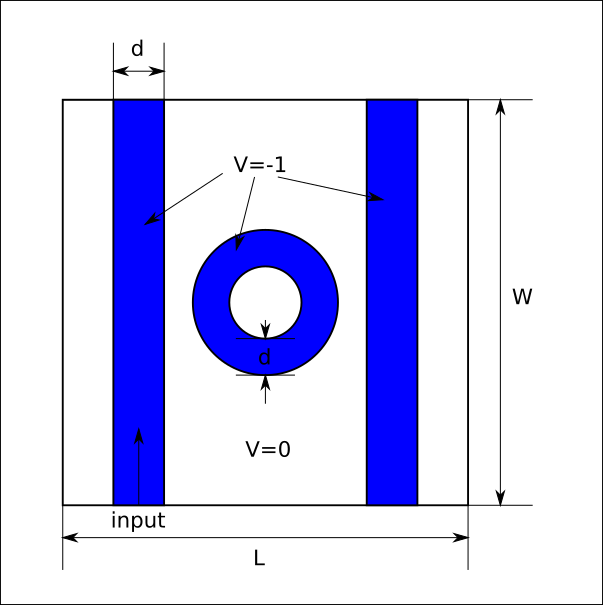
\includegraphics[width=0.5\textwidth]
  {../writeup/sections/intro/system-sketch.png}
  \end{center}

	\item Particle may tunnel to other side of domain
  \end{itemize}
\end{frame}

\begin{frame}{FEM and Variational Form}
  \begin{itemize}
	\item $\Psi \in H^1(\Omega) \times C(\R_+)$
	\item Inner products (bra-ket notation):
			\[
					\bra{\phi}\ket{\psi} = \int_\Omega 
					\phi^* \psi \, dx, \quad 
					\bra{\phi} \mathcal O \ket{\psi} = 
					\int_\Omega \phi^* \mathcal O(\psi) \, dx
			.\] 
	\item Variational form: $\Phi \in H^1_{D, \mathrm{in}}(\Omega)$
			of the Schr\"odinger equation
			\[
			i \bra{\Phi} \partial_t \ket{\Psi} = 
			\bra{\nabla \Phi} \ket{\nabla \Psi} + 
			\bra{\Phi} V \ket{\Psi} + 
			\int_{\Gamma_\mathrm{out}} \Phi \pder{\Psi}{n} \, d\sigma
			\] 
	\item $\Phi$ zero on outer boundary and input boundary, 
			nonzero on other (blue boundaries), wave can escape this way

\end{itemize}
\end{frame}

\begin{frame}{Finite Dimensional FEM}
\begin{itemize} 
		\item Boundary wrapper:
				\[
						B(\Phi, \Psi) = \int_{\Gamma_\mathrm{out}}
						\Phi \pder{\Psi}{n} \, d\sigma
				.\] 
		\item Build triangulation $\mathcal T_h$ on $\Omega$, let 
				$\phi_j(\vec x)$ be a set of basis functions for 
				$H^1_{D, \mathrm{in}}(\Omega)$
			\[\begin{split}
					\implies i \sum_{k=1}^N 
					& \bra{\phi_j} \ket{\phi_k} \lambda_k'(t) = \\
					& \sum_{k=1}^N \left[
					\bra{\nabla \phi_j} \ket{\nabla \phi_k}
	       			+ \bra{\phi_j} V \ket{\phi_k} + 
					B(\phi_j, \phi_k)
			\right] 
					\lambda_k(t)
			\end{split}\] 
	\item Mass matrix: 
			$\bra{\phi_j}\ket{\phi_k}$, 
			Stiffness matrix:
			$\bra{\nabla \phi_j}\ket{\nabla \phi_k}$,
			``Potential'' matrix:
			$\bra{\phi_j} V \ket{\phi_k}$, 
			``Boundary'' matrix:
			$B(\phi_j, \phi_k)$
\end{itemize}
\end{frame}

\begin{frame}{Time Stepping and Solution}
  
\end{frame}
\begin{frame}{References}
		\bibliography{../writeup/biblio.bib}
		\bibliographystyle{alpha}
		\nocite{*}
\end{frame}

\end{document}
